% ============================================================
%  Springer LNCS paper -- IVP Group 19
%  Overleaf: New Project -> Templates -> "Springer Lecture Notes in
%  Computer Science" (gives llncs.cls + splncs04.bst), then replace
%  main.tex with this file.
% ============================================================
\documentclass[runningheads]{llncs}

\usepackage[T1]{fontenc}
\usepackage{graphicx}
\usepackage{amsmath,amssymb}
\usepackage{booktabs}
\usepackage{tabularx}
\usepackage{url}
\usepackage{array}
\usepackage{tikz}
\usetikzlibrary{arrows.meta,positioning,fit,calc,shapes.geometric}

% ---------- TikZ styles used by all flow diagrams ----------
\tikzset{
  blk/.style={rectangle,rounded corners=2pt,draw=black!70,fill=blue!8,
              align=center,minimum height=8mm,inner sep=3pt,font=\scriptsize},
  enc/.style={blk,fill=blue!30},
  fus/.style={blk,fill=pink!70},
  outb/.style={blk,fill=purple!35},
  los/.style={blk,fill=orange!30},
  arr/.style={-{Stealth[length=1.8mm]},thick},
  lab/.style={font=\tiny,align=center,text=black!70}
}

\begin{document}

\title{Multi-view Human Action Recognition: TSN--GRU, Clip-Consistent Augmentation, and Paired-View Temporal Learning}
\titlerunning{Multi-view HAR with Paired-View Temporal Learning}

\author{Vichanshu Raj \and Satwik Santosh \and Vishwas Pahwa \and Sudhanshu \and Kyan Mahajan \and Saumya Sood \and Akshat Parmar}
\authorrunning{V. Raj et al.}

\institute{Group 19, Image and Video Processing (IVP) Course Project\\
Indian Institute of Information Technology, Allahabad, India\\
\email{\{IIT2024083, IIT2024084, IIT2024087, IIT2024081, IIT2024092, IIT2024018, IIT2024077\}@iiita.ac.in}}

\maketitle

\begin{abstract}
Recognising human actions from several synchronised cameras reduces the effect of occlusion, but models trained on some cameras often fail on a camera they have never seen.
We re-implement the multi-branch Temporal Segment Network with a GRU temporal consensus (TSN+GRU) of Bui and Nguyen on the Northwestern-UCLA (N-UCLA) RGB data and evaluate it with cross-subject and cross-view protocols.
A code audit of the baseline identifies three issues: horizontal flips are sampled independently for each snippet, creating inconsistent left--right appearance within a clip; the model over-fits (training accuracy $\approx$92\% against 70--72\% test accuracy); and the held-out view is the most difficult target.
We fix the first problem with \emph{clip-consistent augmentation}, where every random transform is sampled once per clip. This raises cross-view accuracy on the unseen view~3 from 70.8\% to 78.5\%.
We then evaluate a \emph{paired-view-regularized temporal Transformer}: one shared ResNet-18 encoder, eight frames per clip, a two-layer Transformer with attention pooling, and a paired-view cosine consistency loss. This objective encourages agreement across the two training views; invariance to an unseen camera remains an empirical question.
The new model reaches 86.12\% (360/418) on the unseen view with a single input clip.
We describe the architectures with flow diagrams, derive the equations of each component, and report the limits of our evaluation (one cross-subject fold, 12 training epochs).

\keywords{Multi-view action recognition \and Temporal Segment Network \and GRU \and Transformer \and View invariance \and Data augmentation \and N-UCLA.}
\end{abstract}

% =====================================================================
\section{Introduction}
Automatic action recognition is needed wherever camera networks outgrow human operators, for example in CCTV surveillance, smart homes and in-vehicle monitoring~\cite{veesam2025,ma2023}.
A single camera loses evidence through \emph{occlusion} (hands or objects hidden) and through \emph{viewpoint change}: the same action looks different from another angle, so a model trained on one set of cameras transfers poorly to a new camera~\cite{wang2018dana}.
Synchronised cameras provide complementary evidence, and fusing them gives a more robust decision.

Bui and Nguyen~\cite{bui2020} showed that a Temporal Segment Network (TSN)~\cite{wang2016tsn} with one CNN branch per camera and a Gated Recurrent Unit (GRU)~\cite{cho2014} for temporal consensus is a simple and effective multi-view recogniser.
Our work started as a faithful re-implementation of that paper and then moved to the weak points we found.
Our contributions are:
\begin{itemize}
\item A documented, reproducible PyTorch implementation of multi-branch TSN+GRU with four evaluation protocols (cross-subject and three cross-view splits) on N-UCLA.
\item A code audit that identifies a per-frame augmentation bug and a clip-consistent augmentation rule that fixes it (Sect.~\ref{sec:aug}).
\item A paired-view-regularized temporal Transformer that uses one shared model at inference, attention pooling over frames, and a cosine consistency loss during paired-view training (Sect.~\ref{sec:transformer}).
\item An honest account of what is and is not comparable with published results (Sect.~\ref{sec:discussion}).
\end{itemize}
We borrow \emph{ideas} from DVANet~\cite{siddiqui2024}, TBCNet~\cite{yang2026} and cross-view attention~\cite{nguyen2021}; those models are not implemented here.

The paper is organised as follows. Sect.~2 reviews related work, Sect.~3 describes the dataset and protocols, Sect.~4 the baseline, Sect.~5 the augmentation fix, Sect.~6 the Transformer model, Sect.~7 the experiments, and Sects.~8--9 discuss and conclude.

% =====================================================================
\section{Related Work}
We group representative prior work by the nature of the method (Table~\ref{tab:survey}).

\begin{table}[t]
\caption{Literature categories and the ideas we carried into this work.}\label{tab:survey}
\centering
\small
\begin{tabularx}{\textwidth}{@{}p{2.5cm}p{3.4cm}X@{}}
\toprule
Category & Key papers & Idea we used \\
\midrule
Single-view foundations & Two-stream~\cite{simonyan2014}, TSN~\cite{wang2016tsn} & Sparse segment sampling, flip/crop augmentation, partial BN \\
Multi-branch fusion & TSN+GRU~\cite{bui2020} (base), DA-Net~\cite{wang2018dana} & One CNN branch per view, late fusion \\
Attention fusion & Cross-view attention~\cite{nguyen2021} & Learn which evidence matters $\rightarrow$ attention pooling over frames \\
View-invariant learning & ViewCon~\cite{shah2023}, DVANet~\cite{siddiqui2024}, TBCNet~\cite{yang2026} & Same action from two cameras should give the same features $\rightarrow$ paired-view cosine loss \\
Real-world multi-camera & M2DAR~\cite{ma2023}, MultiTSF~\cite{nguyen2025} & Motivation (driver monitoring, smart homes) \\
\bottomrule
\end{tabularx}
\end{table}

\paragraph{Multi-branch TSN with GRU.}
TSN divides a video into $K$ segments and samples one snippet per segment, so the whole action is covered cheaply~\cite{wang2016tsn}. Bui and Nguyen~\cite{bui2020} apply a shared Inception-BN backbone to three synchronised cameras, refine each view with its own $3{\times}3$ convolution, replace the unordered average consensus by a GRU that reads the snippets in temporal order, and concatenate the three view descriptors before a classifier.

\paragraph{Cross-view attention and view invariance.}
Cross-view attention (CVA)~\cite{nguyen2021} lets one camera attend to evidence from the others before classification. DVANet~\cite{siddiqui2024} separates action features from view features with learnable queries in a transformer decoder and contrastive losses, so that the predicted action does not depend on the camera. TBCNet~\cite{yang2026} adds deformable aggregation and trunk--branch contrastive learning.
Table~\ref{tab:evolution} compares the fusion strategies; it is an architecture comparison, not a leaderboard, because the papers differ in modality, backbone, pre-training, protocol and prediction unit.

\begin{table}[t]
\caption{Evolution of multi-view fusion on N-UCLA (architecture comparison only).}\label{tab:evolution}
\centering
\scriptsize
\begin{tabularx}{\textwidth}{@{}p{2.25cm}c X X p{1.65cm}@{}}
\toprule
Method & Year & Temporal representation & Multi-view fusion & Relevance \\
\midrule
TSN+GRU~\cite{bui2020} & 2020 & Sparse segments + GRU & Late concatenation & Our baseline \\
CVA~\cite{nguyen2021} & 2021 & 3-D R(2+1)D features & Attention across camera branches & Learned view interaction \\
DVANet~\cite{siddiqui2024} & 2024 & Spatio-temporal encoder + transformer queries & Action / view disentanglement & View invariance \\
TBCNet~\cite{yang2026} & 2026 & 3-D spatio-temporal features & Deformable aggregation + contrastive & Future direction \\
\textbf{Ours} & 2026 & 8 frames + Transformer + attention pooling & Shared single-view model + paired-view loss & Sect.~\ref{sec:transformer} \\
\bottomrule
\end{tabularx}
\end{table}

\begin{table}[t]
\caption{Published results reported by the original papers on N-UCLA (literature evidence, \emph{not} our results; protocols differ).}\label{tab:published}
\centering
\small
\begin{tabular}{lcc}
\toprule
Paper & Cross-subject (\%) & Cross-view (\%) \\
\midrule
TSN+GRU~\cite{bui2020} & 93.81 & 84.4 (mean) \\
Cross-view attention~\cite{nguyen2021} & up to 99.56 & up to 92.74 \\
DVANet~\cite{siddiqui2024} & 94.4 & 96.5 \\
\bottomrule
\end{tabular}
\end{table}

% =====================================================================
\section{Dataset, Camera Topology and Protocols}
\subsection{Northwestern-UCLA (N-UCLA)}
We use the RGB videos of N-UCLA~\cite{wang2014} from a Kaggle copy that we audited~\cite{raj2026}. Three static, synchronised Kinect cameras with overlapping fields of view record ten daily actions performed by ten subjects (Fig.~\ref{fig:cameras}). Table~\ref{tab:dataset} summarises the data.

\begin{table}[t]
\caption{Properties of the N-UCLA RGB data used in this work.}\label{tab:dataset}
\centering
\small
\begin{tabular}{ll}
\toprule
Property & Value \\
\midrule
Modality & RGB video \\
Videos & 1{,}475 (1.33~GB) \\
Actions / subjects / views & 10 / 10 / 3 \\
Videos per view (view 1 / 2 / 3) & 514 / 501 / 460 \\
Complete 3-view groups & 418 (about 42 per class) \\
Frames per video & median 16 \\
Resolution / frame rate & $640{\times}480$, 12~fps (sample clip) \\
\bottomrule
\end{tabular}
\end{table}

The ten actions are: pick up with one hand, pick up with two hands, drop trash, walk around, sit down, stand up, donning jacket, doffing jacket, throw, and carry. Files are named \texttt{v\#\#\_s\#\#\_e\#\#.avi} (view, subject, episode). A \emph{group} is one action instance seen by all three cameras.

\begin{figure}[t]
\centering
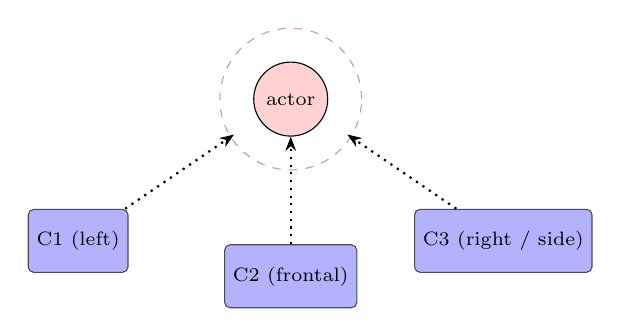
\begin{tikzpicture}[scale=0.9]
  \node[draw,rounded corners,fill=pink!70,circle,minimum size=9mm,font=\scriptsize] (a) at (0,2) {actor};
  \draw[dashed,pink!80!black] (a) circle (1.0);
  \node[enc] (c1) at (-3,0) {C1 (left)};
  \node[enc] (c2) at (0,-0.5) {C2 (frontal)};
  \node[enc] (c3) at (3,0) {C3 (right / side)};
  \draw[arr,dotted] (c1) -- (-0.8,1.5);
  \draw[arr,dotted] (c2) -- (a);
  \draw[arr,dotted] (c3) -- (0.8,1.5);
\end{tikzpicture}
\caption{Top view of the N-UCLA set-up: three fixed cameras with overlapping fields of view all see one action area; the actor faces C2.}\label{fig:cameras}
\end{figure}

\subsection{Evaluation protocols}
\paragraph{Cross-subject (CS).} All three views are used. One subject is held out for testing and the other nine are used for training:
\begin{equation}
\mathrm{Acc}_{CS}=\frac{1}{10}\sum_{s=1}^{10}\mathrm{Acc}\big(\mathcal{D}_{\neg s}\rightarrow\mathcal{D}_{s}\big),
\end{equation}
where $\mathcal{D}_{\neg s}$ is the training data of all subjects except $s$ and $\mathcal{D}_s$ is the test data of subject $s$. In our runs only one fold (subject~1, 51 test groups) is evaluated, whereas the base paper averages ten folds.

\paragraph{Cross-view (CV).} Two views are used for training and the third, \emph{unseen} view for testing:
\begin{equation}
\mathrm{Acc}_{CV}=\frac{1}{3}\sum_{v=1}^{3}\mathrm{Acc}\big(\mathcal{D}^{\{1,2,3\}\setminus v}\rightarrow\mathcal{D}^{v}\big).
\end{equation}
There are three splits ($\rightarrow1$, $\rightarrow2$, $\rightarrow3$) and each has 418 test groups. Because the network has two branches in this setting, the baseline duplicates the single target-view clip into both branches at test time~\cite{bui2020}.

\paragraph{Metrics.} Accuracy and macro-F1 are reported:
\begin{equation}
\mathrm{Acc}=\frac{1}{N}\sum_{n=1}^{N}\mathbf{1}[\hat y_n=y_n],\qquad
\text{Macro-F1}=\frac{1}{C}\sum_{c=1}^{C}\frac{2P_cR_c}{P_c+R_c},
\end{equation}
where $N$ is the number of test groups, $\mathbf 1[\cdot]$ is the indicator function, $C=10$ is the number of classes and $P_c$, $R_c$ are the precision and recall of class $c$. Accuracy counts every test sample equally; macro-F1 gives every class the same weight, so it is lower than accuracy when some classes are weak.

% =====================================================================
\section{Baseline: Multi-branch TSN with GRU Consensus}
\subsection{Data pipeline}
Fig.~\ref{fig:pipeline} shows the pipeline: inventory $\rightarrow$ grouping $\rightarrow$ protocol split $\rightarrow$ segment sampling $\rightarrow$ pre-processing.

\begin{figure}[t]
\centering
\resizebox{\textwidth}{!}{%
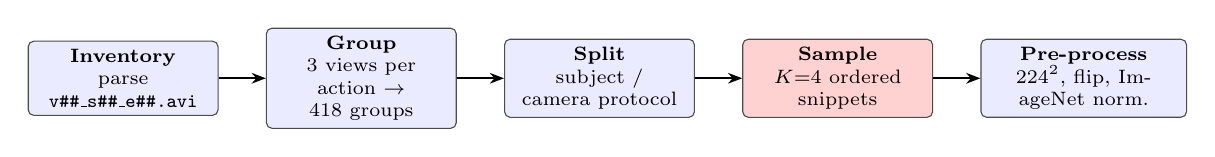
\begin{tikzpicture}[node distance=6mm]
  \node[blk,text width=2.2cm] (n1) {\textbf{Inventory}\\parse \texttt{v\#\#\_s\#\#\_e\#\#.avi}};
  \node[blk,text width=2.2cm,right=of n1] (n2) {\textbf{Group}\\3 views per action $\rightarrow$ 418 groups};
  \node[blk,text width=2.2cm,right=of n2] (n3) {\textbf{Split}\\subject / camera protocol};
  \node[fus,text width=2.2cm,right=of n3] (n4) {\textbf{Sample}\\$K{=}4$ ordered snippets};
  \node[blk,text width=2.4cm,right=of n4] (n5) {\textbf{Pre-process}\\$224^2$, flip, ImageNet norm.};
  \foreach \a/\b in {n1/n2,n2/n3,n3/n4,n4/n5} \draw[arr] (\a)--(\b);
\end{tikzpicture}}
\caption{Data pipeline of the baseline.}\label{fig:pipeline}
\end{figure}

\paragraph{Segment sampling.}
A video of $T$ frames is cut into $K$ equal segments
\begin{equation}
S_k=\Big[\Big\lfloor\tfrac{(k-1)T}{K}\Big\rfloor,\ \Big\lfloor\tfrac{kT}{K}\Big\rfloor-1\Big],\quad k=1,\dots,K,
\end{equation}
and one frame index $t_k$ is taken from each segment:
\begin{equation}
t_k\sim\mathcal{U}(S_k)\ \ \text{(training)},\qquad t_k=\Big\lfloor\tfrac{\min S_k+\max S_k}{2}\Big\rfloor\ \ \text{(test)}.
\end{equation}
Random sampling during training acts as temporal-jitter augmentation, while the deterministic segment centre makes testing repeatable. Example: for $T=16$ and $K=4$ the segments are frames 0--3, 4--7, 8--11 and 12--15, and the test frames are 1, 5, 9 and 13. Sampling in segment order keeps the temporal order of the snippets, which the GRU needs.

\subsection{Architecture}
Fig.~\ref{fig:baseline} shows the baseline. For each view $v\in\{1,\dots,V\}$ the $K$ snippets pass through one \emph{shared} Inception-v3 trunk (ImageNet initialisation~\cite{szegedy2016}), giving a $2048{\times}5{\times}5$ map per snippet. A view-specific block (Conv $3{\times}3$, BatchNorm, ReLU, global average pooling) reduces it to a 256-D vector $\mathbf q^{v}_k$. A GRU shared across views reads $\mathbf q^{v}_1,\dots,\mathbf q^{v}_K$ in order and its last hidden state is the view descriptor.

\begin{figure}[t]
\centering
\resizebox{\textwidth}{!}{%
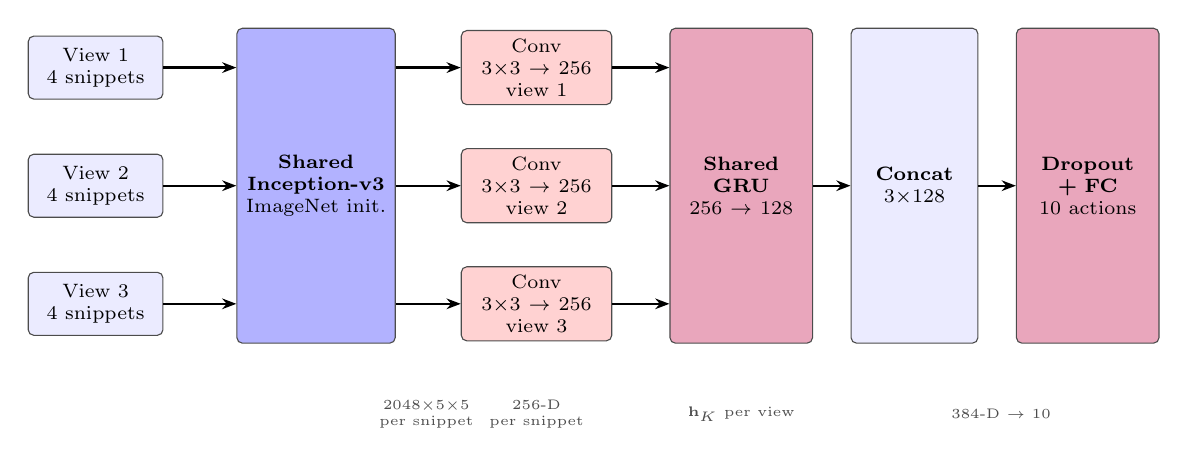
\begin{tikzpicture}
  \node[blk,text width=1.5cm] (v1) at (0,1.5) {View 1\\4 snippets};
  \node[blk,text width=1.5cm] (v2) at (0,0)   {View 2\\4 snippets};
  \node[blk,text width=1.5cm] (v3) at (0,-1.5){View 3\\4 snippets};
  \node[enc,text width=1.8cm,minimum height=4cm] (inc) at (2.8,0) {\textbf{Shared Inception-v3}\\ImageNet init.};
  \node[fus,text width=1.7cm] (c1) at (5.6,1.5) {Conv $3{\times}3\rightarrow256$\\view 1};
  \node[fus,text width=1.7cm] (c2) at (5.6,0)   {Conv $3{\times}3\rightarrow256$\\view 2};
  \node[fus,text width=1.7cm] (c3) at (5.6,-1.5){Conv $3{\times}3\rightarrow256$\\view 3};
  \node[outb,text width=1.6cm,minimum height=4cm] (gru) at (8.2,0) {\textbf{Shared GRU}\\$256\rightarrow128$};
  \node[blk,text width=1.4cm,minimum height=4cm] (cat) at (10.4,0) {\textbf{Concat}\\$3{\times}128$};
  \node[outb,text width=1.6cm,minimum height=4cm] (fc) at (12.6,0) {\textbf{Dropout + FC}\\10 actions};
  \foreach \v/\c in {v1/c1,v2/c2,v3/c3} {
     \draw[arr] (\v.east) -- (\v.east -| inc.west);
     \draw[arr] (inc.east |- \c) -- (\c.west);
     \draw[arr] (\c.east) -- (\c.east -| gru.west);
  }
  \draw[arr] (gru.east) -- (cat.west);
  \draw[arr] (cat.east) -- (fc.west);
  \node[lab] at (4.2,-2.9) {$2048{\times}5{\times}5$\\per snippet};
  \node[lab] at (5.6,-2.9) {256-D\\per snippet};
  \node[lab] at (8.2,-2.9) {$\mathbf h_K$ per view};
  \node[lab] at (11.5,-2.9) {384-D $\rightarrow$ 10};
\end{tikzpicture}}
\caption{Baseline multi-branch TSN+GRU (adapted from~\cite{bui2020}). The trunk and the GRU are shared across views; each view has its own refinement convolution.}\label{fig:baseline}
\end{figure}

\subsection{The GRU consensus explained}
Average consensus takes the unordered mean of the snippet features and ignores the order of events. A GRU~\cite{cho2014} reads the snippets one by one (Fig.~\ref{fig:gru}) and decides at every step how much of the past to keep. With input $\mathbf x_t=\mathbf q_t$ and previous state $\mathbf h_{t-1}$:
\begin{align}
\mathbf z_t &= \sigma(\mathbf W_z\mathbf x_t+\mathbf U_z\mathbf h_{t-1}+\mathbf b_z) &&\text{(update gate)}\\
\mathbf r_t &= \sigma(\mathbf W_r\mathbf x_t+\mathbf U_r\mathbf h_{t-1}+\mathbf b_r) &&\text{(reset gate)}\\
\tilde{\mathbf h}_t &= \tanh\!\big(\mathbf W_h\mathbf x_t+\mathbf U_h(\mathbf r_t\odot\mathbf h_{t-1})+\mathbf b_h\big) &&\text{(candidate state)}\\
\mathbf h_t &= (1-\mathbf z_t)\odot\mathbf h_{t-1}+\mathbf z_t\odot\tilde{\mathbf h}_t &&\text{(new state)}
\end{align}
Here $\sigma$ is the sigmoid function and $\odot$ is element-wise multiplication. The update gate $\mathbf z_t$ chooses between keeping the old state ($\mathbf z_t\to0$) and writing the new candidate ($\mathbf z_t\to1$). The reset gate $\mathbf r_t$ decides how much of the past is used to form the candidate. The final state $\mathbf h_K$ is the descriptor of the view. Because the GRU depends on the order of its inputs, \emph{all snippets of a clip must receive the same augmentation} (Sect.~\ref{sec:aug}).

\begin{figure}[t]
\centering
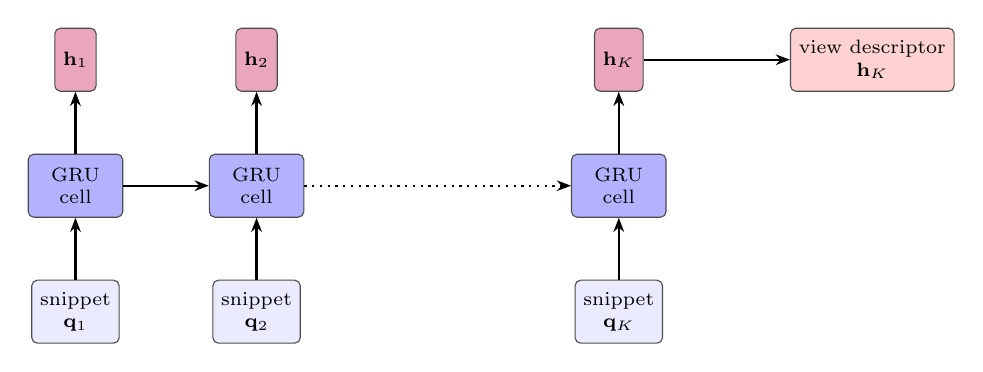
\begin{tikzpicture}[x=2.3cm,y=1cm]
  \foreach \i/\l in {0/1,1/2,3/K} {
    \node[blk] (x\i) at (\i,0) {snippet\\$\mathbf q_{\l}$};
    \node[enc,minimum width=1.2cm] (g\i) at (\i,1.6) {GRU\\cell};
    \node[outb] (h\i) at (\i,3.2) {$\mathbf h_{\l}$};
    \draw[arr] (x\i)--(g\i);
    \draw[arr] (g\i)--(h\i);
  }
  \draw[arr] (g0)--(g1);
  \draw[arr,dotted] (g1)--(g3);
  \node[fus] (f) at (4.4,3.2) {view descriptor\\$\mathbf h_K$};
  \draw[arr] (h3)--(f);
\end{tikzpicture}
\caption{GRU consensus: snippets are read in temporal order and only the last state $\mathbf h_K$ is passed on (adapted from~\cite{bui2020}).}\label{fig:gru}
\end{figure}

\subsection{Fusion, classification and loss}
The descriptors of the $V$ views are concatenated and classified:
\begin{equation}
\mathbf f=\big[\mathbf h^{1}_{K}\,\|\,\mathbf h^{2}_{K}\,\|\,\dots\,\|\,\mathbf h^{V}_{K}\big]\in\mathbb R^{V\cdot128},\qquad
\hat{\mathbf y}=\mathrm{softmax}\big(\mathbf W_c\,\mathrm{Drop}_{0.5}(\mathbf f)+\mathbf b_c\big),
\end{equation}
where $\|$ is concatenation and $\mathrm{Drop}_{0.5}$ randomly zeroes half of the entries during training to reduce over-fitting. Training minimises the cross-entropy over a batch of $B$ groups,
\begin{equation}
\mathcal L_{CE}=-\frac1B\sum_{b=1}^{B}\log\frac{\exp(s_{b,y_b})}{\sum_{c=1}^{10}\exp(s_{b,c})},
\end{equation}
where $s_{b,c}$ is the logit of class $c$ for sample $b$ and $y_b$ is its true class. The model has about 36.1\,M parameters for $V{=}3$ (CS) and 31.4\,M for $V{=}2$ (CV). The tensor shapes are listed in Table~\ref{tab:shapes}.

\begin{table}[t]
\caption{Tensor shapes of the baseline in the cross-view setting ($V{=}2$, $K{=}4$).}\label{tab:shapes}
\centering
\small
\begin{tabular}{lll}
\toprule
Stage & Output shape & Component \\
\midrule
Input & $B\times2\times4\times3\times224^2$ & views $\times$ snippets \\
Shared trunk & $2048\times5\times5$ per snippet & Inception-v3 \\
View branch & 256-D per snippet & Conv $3{\times}3$ + BN + ReLU + GAP \\
Temporal & $\mathbf h_K\in\mathbb R^{128}$ per view & \texttt{nn.GRU(256,128)}, shared \\
Fusion & 256-D & concat + dropout 0.5 \\
Classifier & 10 logits & Linear \\
\bottomrule
\end{tabular}
\end{table}

\subsection{Training set-up}
Table~\ref{tab:setup} compares our run with the base paper. We use the same learning-rate schedule shape but only 12 epochs instead of 80, a different backbone (Inception-v3 instead of Inception-BN) and a single cross-subject fold. All Kaggle runs use SGD (momentum 0.9, weight decay $5{\times}10^{-4}$, learning rate $10^{-3}$, batch of 2 groups, \texttt{MultiStepLR} with milestones at epochs 4 and 9 and $\gamma{=}0.1$), seed 42, and save split manifests and per-epoch logs.

\begin{table}[t]
\caption{Training set-up: base paper versus our baseline run.}\label{tab:setup}
\centering
\small
\begin{tabular}{lll}
\toprule
Setting & Base paper~\cite{bui2020} & Our run \\
\midrule
Epochs & 80 & 12 \\
Learning rate & 0.001, $\div10$ twice & 0.001, $\div10$ twice \\
Backbone & Inception-BN & Inception-v3 \\
Augmentation & crop + scale jitter & horizontal flip \\
Cross-subject folds & 10 & 1 (subject 1) \\
Hardware & GTX 1080 & Kaggle Tesla T4 \\
\bottomrule
\end{tabular}
\end{table}

% =====================================================================
\section{Code Audit and Clip-Consistent Augmentation}\label{sec:aug}
\subsection{Why the baseline plateaued}
After the first runs we audited the code and the learning curves and found three causes of the plateau (Fig.~\ref{fig:audit}).

\begin{figure}[t]
\centering
\resizebox{\textwidth}{!}{%
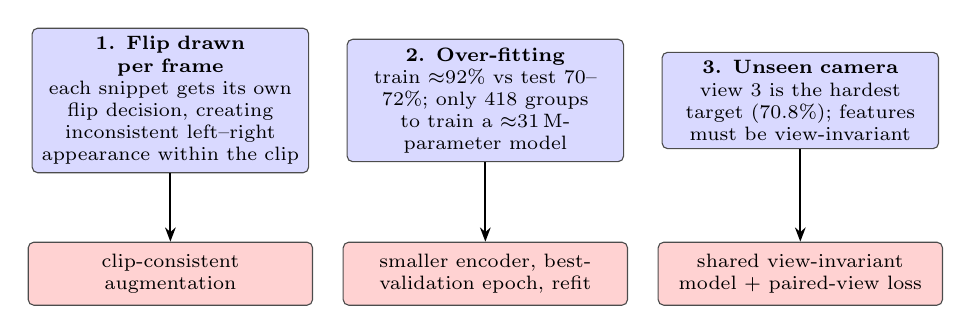
\begin{tikzpicture}
  \node[blk,text width=3.3cm,fill=blue!15] (a) at (0,0) {\textbf{1. Flip drawn per frame}\\each snippet gets its own flip decision, creating inconsistent left--right appearance within the clip};
  \node[blk,text width=3.3cm,fill=blue!15] (b) at (4,0) {\textbf{2. Over-fitting}\\train $\approx$92\% vs test 70--72\%; only 418 groups to train a $\approx$31\,M-parameter model};
  \node[blk,text width=3.3cm,fill=blue!15] (c) at (8,0) {\textbf{3. Unseen camera}\\view 3 is the hardest target (70.8\%); features must be view-invariant};
  \node[fus,text width=3.4cm] (fa) at (0,-2.2) {clip-consistent augmentation};
  \node[fus,text width=3.4cm] (fb) at (4,-2.2) {smaller encoder, best-validation epoch, refit};
  \node[fus,text width=3.4cm] (fc) at (8,-2.2) {shared view-invariant model + paired-view loss};
  \draw[arr] (a)--(fa); \draw[arr] (b)--(fb); \draw[arr] (c)--(fc);
\end{tikzpicture}}
\caption{Findings of the code audit and the fix chosen for each.}\label{fig:audit}
\end{figure}

\paragraph{Per-frame flip.} In the baseline the random flip was inside the snippet loop (a new coin toss for each frame). This does not change the temporal order of the snippets, but it can make the actor's orientation switch inconsistently between samples. A recurrent model may then receive artificial appearance changes unrelated to the action. The fix draws the random variable once per clip:
\begin{verbatim}
flip = train and random.random() < .5     # one draw per clip
for idx in ids:                           # 4 ordered snippets
    im = cv2.resize(rgb(frame[idx]), (224, 224))
    if flip: im = im[:, ::-1]             # same for all 4 frames
\end{verbatim}
\textbf{Rule adopted:} every random transform is sampled once per clip and applied identically to all $K$ snippets.

\subsection{Augmentation policy}
Besides the flip, a photometric jitter mimics exposure differences between cameras. For a pixel value $I$ the augmented value is
\begin{equation}
I'=\mathrm{clip}\big(\alpha I+\beta,\,0,\,255\big),\qquad \alpha\sim\mathcal U(0.9,1.1),\ \ \beta\sim\mathcal U(-8,8),
\end{equation}
where $\alpha$ changes contrast, $\beta$ changes brightness, and $\mathrm{clip}$ keeps the result in the valid range. The pair $(\alpha,\beta)$ is applied with probability 0.5 and is drawn once per clip. Table~\ref{tab:aug} lists the policy. Each camera view is read separately, so each view receives its own draw. No random augmentation is used at validation or test time. The same photometric step is a reusable module for the BN-Inception variant (BGR input, no flip).

\begin{table}[t]
\caption{Clip-consistent augmentation policy ($K{=}4$ snippets per view).}\label{tab:aug}
\centering
\small
\begin{tabular}{lll}
\toprule
Transform & Range / probability & Sampled \\
\midrule
Horizontal flip & $p=0.5$ & once per clip \\
Contrast $\alpha$ & $0.9$--$1.1$, $p=0.5$ & once per clip \\
Brightness $\beta$ & $-8\ldots+8$ & same draw as $\alpha$ \\
Temporal jitter & random frame in each segment & per segment \\
\bottomrule
\end{tabular}
\end{table}

\subsection{Experiment protocol: develop, refit, test once}
To avoid tuning on the test view we use the protocol of Fig.~\ref{fig:protocol}: views~1 and~2 are used for training and view~3 is held out. In the \emph{development} stage the model is trained on subjects 1--9 (375 pairs) and validated on subject~10 (43 pairs). It is then \emph{refit} from scratch on all 418 view-1+2 pairs with the same schedule, and \emph{tested once} on all 418 view-3 clips.

\begin{figure}[t]
\centering
\resizebox{\textwidth}{!}{%
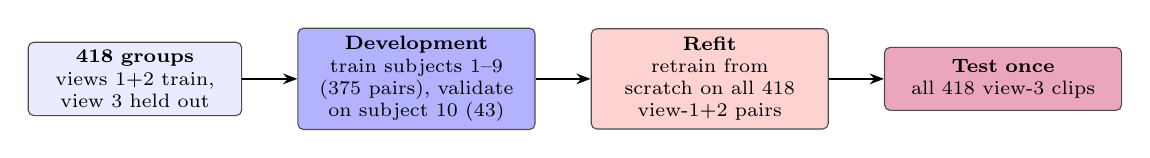
\begin{tikzpicture}[node distance=7mm]
  \node[blk,text width=2.5cm] (g) {\textbf{418 groups}\\views 1+2 train,\\view 3 held out};
  \node[enc,text width=2.8cm,right=of g] (d) {\textbf{Development}\\train subjects 1--9 (375 pairs), validate on subject 10 (43)};
  \node[fus,text width=2.8cm,right=of d] (r) {\textbf{Refit}\\retrain from scratch on all 418 view-1+2 pairs};
  \node[outb,text width=2.8cm,right=of r] (t) {\textbf{Test once}\\all 418 view-3 clips};
  \foreach \a/\b in {g/d,d/r,r/t} \draw[arr] (\a)--(\b);
\end{tikzpicture}}
\caption{Develop, refit, test once.}\label{fig:protocol}
\end{figure}

% =====================================================================
\section{Paired-View-Regularized Temporal Transformer}\label{sec:transformer}
The error analysis (Sect.~\ref{sec:results}) shows that locomotion classes from a new viewpoint and the train/test gap are the main failures. We therefore redesigned the model around three ideas: one shared single-view model, a temporal Transformer in place of the GRU, and a loss that pulls paired camera views together (Fig.~\ref{fig:improved}).

\begin{figure}[t]
\centering
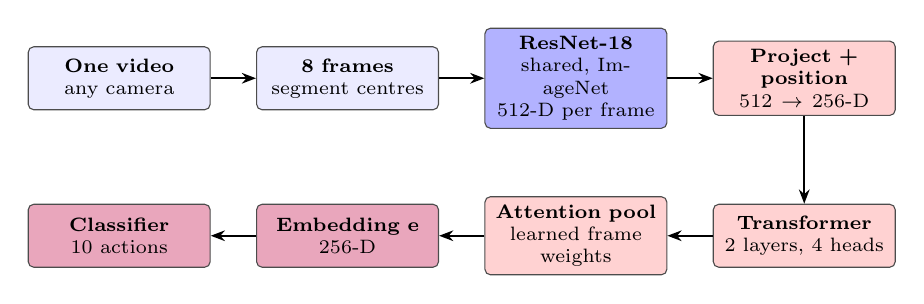
\begin{tikzpicture}[x=1cm,y=1cm]
  \node[blk,text width=2.1cm] (n1) at (0,0)   {\textbf{One video}\\any camera};
  \node[blk,text width=2.1cm] (n2) at (2.9,0) {\textbf{8 frames}\\segment centres};
  \node[enc,text width=2.1cm] (n3) at (5.8,0) {\textbf{ResNet-18}\\shared, ImageNet\\512-D per frame};
  \node[fus,text width=2.1cm] (n4) at (8.7,0) {\textbf{Project + position}\\$512\rightarrow256$-D};
  \node[fus,text width=2.1cm] (n5) at (8.7,-2) {\textbf{Transformer}\\2 layers, 4 heads};
  \node[fus,text width=2.1cm] (n6) at (5.8,-2) {\textbf{Attention pool}\\learned frame weights};
  \node[outb,text width=2.1cm] (n7) at (2.9,-2) {\textbf{Embedding} $\mathbf e$\\256-D};
  \node[outb,text width=2.1cm] (n8) at (0,-2)   {\textbf{Classifier}\\10 actions};
  \draw[arr] (n1)--(n2); \draw[arr] (n2)--(n3); \draw[arr] (n3)--(n4);
  \draw[arr] (n4)--(n5); \draw[arr] (n5)--(n6); \draw[arr] (n6)--(n7); \draw[arr] (n7)--(n8);
\end{tikzpicture}
\caption{Inference pipeline of the improved model. One clip from one camera produces one action label; there is no duplication into two branches.}\label{fig:improved}
\end{figure}

\subsection{Frame encoder and temporal Transformer}
Eight frames at segment centres are encoded by a shared ImageNet-pretrained ResNet-18~\cite{he2016}, giving $\mathbf p_k\in\mathbb R^{512}$. Each feature is projected to $d=256$ and a position embedding is added so that the Transformer knows the frame order:
\begin{equation}
\mathbf u_k=\mathbf W_p\mathbf p_k+\mathbf b_p+\mathbf e^{\mathrm{pos}}_k,\qquad k=1,\dots,8.
\end{equation}
The matrix $\mathbf U=[\mathbf u_1;\dots;\mathbf u_8]$ passes through two Transformer encoder layers with four heads~\cite{vaswani2017}. Each head computes scaled dot-product self-attention:
\begin{equation}
\mathrm{Attn}(\mathbf Q,\mathbf K,\mathbf V)=\mathrm{softmax}\!\Big(\frac{\mathbf Q\mathbf K^{\top}}{\sqrt{d_k}}\Big)\mathbf V,\qquad d_k=\frac{d}{4}=64,
\end{equation}
where $\mathbf Q=\mathbf U\mathbf W^Q$, $\mathbf K=\mathbf U\mathbf W^K$, $\mathbf V=\mathbf U\mathbf W^V$ are learned projections of the frame features. Every frame can therefore attend to every other frame, so non-adjacent phases of an action (for example the arm swing at the start and the release at the end of a throw) are linked directly. A GRU, in contrast, passes information only through its recurrent state. The division by $\sqrt{d_k}$ keeps the dot products from growing with the dimension, which would saturate the softmax. The output is a sequence $\mathbf z_1,\dots,\mathbf z_8$.

\subsection{Attention pooling}
The GRU of the baseline keeps only its last step. We instead let the model decide which frames matter. A scalar score is computed for each frame, the scores are normalised with a softmax and the frames are averaged with these weights:
\begin{equation}
s_k=\mathbf w^{\top}\tanh(\mathbf W_a\mathbf z_k+\mathbf b_a),\qquad
\alpha_k=\frac{\exp(s_k)}{\sum_{j=1}^{8}\exp(s_j)},\qquad
\mathbf e=\sum_{k=1}^{8}\alpha_k\mathbf z_k,
\end{equation}
where $\alpha_k\ge0$, $\sum_k\alpha_k=1$, and $\mathbf e\in\mathbb R^{256}$ is the clip embedding. Informative frames receive large $\alpha_k$ and uninformative frames (for example an empty scene before the actor moves) are down-weighted. The logits are $\mathbf s=\mathbf W_c\mathbf e+\mathbf b_c$. This is the same idea as cross-view attention~\cite{nguyen2021}, applied over time instead of over cameras. (The equation above is the standard additive-attention form; the exact parametrisation is in the code repository~\cite{ivprepo}.)

\subsection{Paired-view consistency loss}
During training, view~1 and view~2 of the same event pass through the \emph{same} network (Fig.~\ref{fig:training}) and give embeddings $\mathbf e^{(1)}$, $\mathbf e^{(2)}$ and logits $\mathbf s^{(1)}$, $\mathbf s^{(2)}$. The loss has two parts:
\begin{equation}
\mathcal L=\underbrace{\frac12\sum_{i=1}^{2}\mathcal L^{\varepsilon}_{CE}\big(\mathbf s^{(i)},y\big)}_{\text{classify both views}}
+\lambda\underbrace{\Big(1-\frac{\mathbf e^{(1)\top}\mathbf e^{(2)}}{\|\mathbf e^{(1)}\|\,\|\mathbf e^{(2)}\|}\Big)}_{\text{consistency}},\qquad \lambda=0.1 .
\end{equation}
The first term is the cross-entropy with label smoothing $\varepsilon=0.05$: the target distribution is $q_c=(1-\varepsilon)\,\mathbf 1[c=y]+\varepsilon/C$, which discourages over-confident predictions on a small data set. The second term is one minus the cosine similarity of the two embeddings. It is 0 when the embeddings point in the same direction and grows as they diverge, so the network is pushed to give the same representation to the same event seen by two cameras. This is the idea of keeping action features stable across views from DVANet~\cite{siddiqui2024} and of contrastive alignment from TBCNet~\cite{yang2026}, reduced to a simple pairwise term (we do not implement the disentangling decoder or negative pairs of those models).

\begin{figure}[t]
\centering
\resizebox{\textwidth}{!}{%
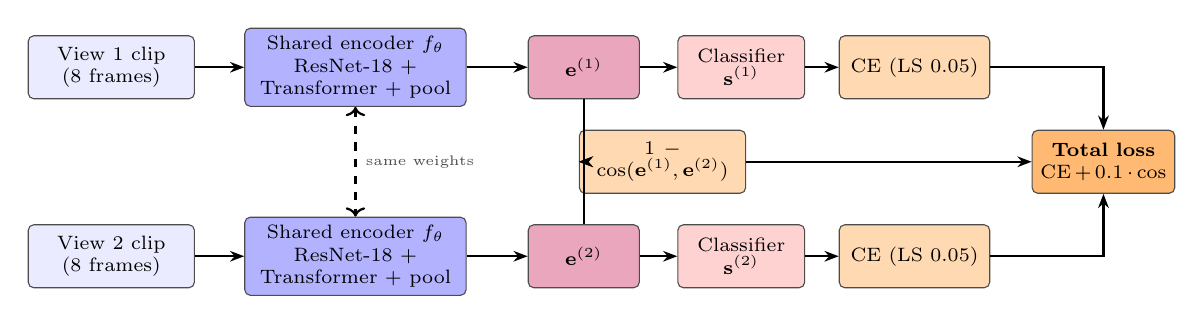
\begin{tikzpicture}
  \node[blk,text width=1.9cm] (v1) at (0,1.2) {View 1 clip\\(8 frames)};
  \node[blk,text width=1.9cm] (v2) at (0,-1.2) {View 2 clip\\(8 frames)};
  \node[enc,text width=2.6cm] (f1) at (3.1,1.2) {Shared encoder $f_\theta$\\ResNet-18 + Transformer + pool};
  \node[enc,text width=2.6cm] (f2) at (3.1,-1.2) {Shared encoder $f_\theta$\\ResNet-18 + Transformer + pool};
  \draw[dashed,<->,thick] (f1.south) -- node[right,lab]{same weights} (f2.north);
  \node[outb,text width=1.2cm] (e1) at (6.0,1.2) {$\mathbf e^{(1)}$};
  \node[outb,text width=1.2cm] (e2) at (6.0,-1.2) {$\mathbf e^{(2)}$};
  \node[fus,text width=1.4cm] (s1) at (8.0,1.2) {Classifier\\$\mathbf s^{(1)}$};
  \node[fus,text width=1.4cm] (s2) at (8.0,-1.2) {Classifier\\$\mathbf s^{(2)}$};
  \node[los,text width=1.7cm] (ce1) at (10.2,1.2) {CE (LS 0.05)};
  \node[los,text width=1.7cm] (ce2) at (10.2,-1.2) {CE (LS 0.05)};
  \node[los,text width=1.9cm] (cos) at (7.0,0) {$1-\cos(\mathbf e^{(1)},\mathbf e^{(2)})$};
  \node[los,text width=1.6cm,fill=orange!55] (tot) at (12.6,0) {\textbf{Total loss}\\$\mathrm{CE}+0.1\cdot\mathrm{cos}$};
  \draw[arr] (v1)--(f1); \draw[arr] (v2)--(f2);
  \draw[arr] (f1)--(e1); \draw[arr] (f2)--(e2);
  \draw[arr] (e1)--(s1); \draw[arr] (e2)--(s2);
  \draw[arr] (s1)--(ce1); \draw[arr] (s2)--(ce2);
  \draw[arr] (e1.south) |- (cos.west);
  \draw[arr] (e2.north) |- (cos.west);
  \draw[arr] (ce1.east) -| (tot.north);
  \draw[arr] (ce2.east) -| (tot.south);
  \draw[arr] (cos.east) -- ++(1.0,0) |- (tot.west);
\end{tikzpicture}}
\caption{Training with paired source views. Both views go through the same network; the loss adds a cosine consistency term to the classification loss. At test time only the unseen view-3 clip is fed in, once.}\label{fig:training}
\end{figure}

\subsection{Differences from the baseline}
Table~\ref{tab:compare} summarises the changes and the reason for each. Note that several things change at once, so the gain cannot yet be attributed to a single component (see Sect.~\ref{sec:discussion}).

\begin{table}[t]
\caption{Baseline versus improved model.}\label{tab:compare}
\centering
\scriptsize
\begin{tabularx}{\textwidth}{@{}p{1.7cm}p{2.5cm}p{2.8cm}X@{}}
\toprule
Aspect & Baseline (TSN+GRU) & Improved model & Reason \\
\midrule
Frame encoder & Inception-v3 & ResNet-18 & smaller model, less over-fitting on 418 groups \\
Frames per clip & 4 & 8 & more motion phases for walk, carry, throw \\
Temporal model & GRU, last step & Transformer + attention pooling & links non-adjacent frames, learns which frames matter \\
Cameras & two branches + concat & one shared model used per view & one representation for every camera \\
Unseen view & clip copied into both branches & single clip, used once & test input matches what the model sees \\
Objective & cross-entropy & + paired-view cosine loss & same event from two cameras should embed alike \\
Epoch choice & fixed 12 epochs & best validation epoch, then refit & less over-training \\
\bottomrule
\end{tabularx}
\end{table}

% =====================================================================
\section{Experiments and Results}\label{sec:results}
\subsection{Implementation and acceptance tests}
All code is written in PyTorch~\cite{paszke2019} with torchvision and OpenCV, and runs on a Kaggle Tesla T4 GPU (PyTorch 2.11, CUDA 12.8). The Software Requirements Specification defines eight functional requirements (dataset validation, group and split construction, segment sampling, training of average and GRU variants, view fusion, checkpoint loading, protocol evaluation, metadata logging) and nine acceptance tests (Table~\ref{tab:tests}). A desktop demo (Tkinter) loads the refit baseline checkpoint, samples four frames at segment centres, feeds the clip to both branches and overlays the predicted action on the video; it can export an annotated MP4.

\begin{table}[t]
\caption{Acceptance tests and status.}\label{tab:tests}
\centering
\small
\begin{tabular}{llll}
\toprule
ID & Test & Status & Evidence \\
\midrule
T01 & Bad input rejected & Partial & -- \\
T02 & Splits are disjoint & Met & holds by construction \\
T03 & $K$ ordered indices & Met & holds by construction \\
T04 & Finite loss, $B{\times}10$ logits & Met & loss 2.13 $\rightarrow$ 0.41 in run log \\
T05 & Checkpoint reload & Met & demo reloads strictly \\
T06 & Wrong branch count & Pending & -- \\
T07 & Metric correctness & Met & recomputed from saved predictions \\
T08 & Run metadata saved & Met & manifests, histories, metrics \\
T09 & Latency / VRAM & Pending & -- \\
\bottomrule
\end{tabular}
\end{table}

\subsection{Baseline results}
Table~\ref{tab:baseline} reports the 12-epoch baseline on the four protocols together with the numbers published in the base paper. The pipeline runs end to end for all four protocols in about 46 minutes.

\begin{table}[t]
\caption{Baseline results (12 epochs) against the base paper~\cite{bui2020}. The base paper uses 80 epochs and averages ten CS folds; we evaluate one.}\label{tab:baseline}
\centering
\small
\begin{tabular}{lccc}
\toprule
Protocol & Acc.\ (\%) ours & Macro-F1 ours & Acc.\ (\%) paper \\
\midrule
Cross-subject (subject 1) & 94.2 & 0.88 & 93.81 \\
Cross-view $\rightarrow$1 & 81.3 & 0.79 & 82.58 \\
Cross-view $\rightarrow$2 & 83.4 & 0.81 & 81.00 \\
Cross-view $\rightarrow$3 & 70.8 & 0.695 & 89.76 \\
\bottomrule
\end{tabular}
\end{table}

\subsection{Progression on the unseen view~3}
Table~\ref{tab:progress} and Fig.~\ref{fig:progress} show the effect of each stage on the cross-view $\{1,2\}\rightarrow3$ protocol.
Clip-consistent augmentation alone gives $+7.7$ points (296/418 to 328/418 correct). The improved architecture reaches 360/418 (86.12\%), a further $+7.6$ points and $+15.3$ points over the baseline.

\begin{table}[t]
\caption{Cross-view $\{1,2\}\rightarrow3$ on all 418 test clips.}\label{tab:progress}
\centering
\small
\begin{tabular}{lccc}
\toprule
Stage & Accuracy (\%) & Macro-F1 & Correct / 418 \\
\midrule
Baseline (Inception-v3, 12 epochs) & 70.8 & 0.695 & 296 \\
+ Clip-consistent augmentation & 78.5 & 0.784 & 328 \\
+ ResNet-18, Transformer, paired-view loss & 86.12 & 0.83 & 360 \\
\midrule
Base paper~\cite{bui2020} (80 epochs, different protocol unit) & 89.76 & -- & -- \\
\bottomrule
\end{tabular}
\end{table}

\begin{figure}[t]
\centering
\resizebox{\textwidth}{!}{%
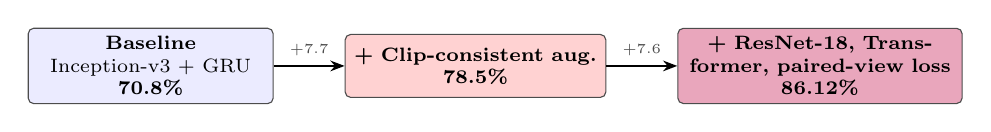
\begin{tikzpicture}[node distance=9mm]
  \node[blk,text width=2.9cm] (a) {\textbf{Baseline}\\Inception-v3 + GRU\\\textbf{70.8\%}};
  \node[fus,text width=3.1cm,right=of a] (b) {\textbf{+ Clip-consistent aug.}\\\textbf{78.5\%}};
  \node[outb,text width=3.4cm,right=of b] (c) {\textbf{+ ResNet-18, Transformer, paired-view loss}\\\textbf{86.12\%}};
  \draw[arr] (a) -- node[above,lab]{+7.7} (b);
  \draw[arr] (b) -- node[above,lab]{+7.6} (c);
\end{tikzpicture}}
\caption{Accuracy on the unseen view~3 after each stage.}\label{fig:progress}
\end{figure}

\subsection{Error analysis on the unseen view}
Table~\ref{tab:perclass} gives the per-class recall of the augmentation run (overall 78.5\%). \emph{Sit down} transfers best because its large vertical posture change looks similar from every camera. \emph{Donning} and \emph{doffing} a jacket are confused with each other (10 and 11 swaps), as they are almost time-reversed versions of one another. The locomotion classes \emph{walk around} and \emph{carry} are the weakest and are the most sensitive to viewpoint and dynamic occlusion; carrying an object is confused with walking with free arms. These failures motivated the Transformer (more frames, direct links between distant frames) and the paired-view loss.

\begin{table}[t]
\caption{Per-class recall on the unseen view~3 for the clip-consistent augmentation run (Inception-v3).}\label{tab:perclass}
\centering
\small
\begin{tabular}{lcc}
\toprule
Class & Recall (\%) & Correct / total \\
\midrule
Sit down & 90.7 & 39/43 \\
Stand up & 82.2 & 37/45 \\
Pick up (1 hand) & 78.6 & 33/42 \\
Drop trash & 77.8 & 28/36 \\
Donning jacket & 76.7 & 33/43 \\
Doffing jacket & 76.7 & 33/43 \\
Pick up (2 hands) & 76.7 & 33/43 \\
Walk around & 75.6 & 34/45 \\
Throw & 75.0 & 30/40 \\
Carry & 73.7 & 28/38 \\
\bottomrule
\end{tabular}
\end{table}

% =====================================================================
\section{Discussion and Limitations}\label{sec:discussion}
\paragraph{Comparison with published numbers.} Published results (Table~\ref{tab:published}) come from different protocols, back-bones, initialisation, prediction units and training lengths. Our 12-epoch, single-fold runs are therefore not a reproduction of those numbers, and we do not claim to beat any published method.

\paragraph{Attribution.} The improved model changes the encoder, the number of frames, the temporal model, the objective and the epoch selection at once. We have not yet run the single-component ablations (for example Transformer without the cosine loss) that would show which change gives the gain.

\paragraph{Statistical confidence.} Each cross-view split has 418 test groups, so one clip is about 0.24 percentage points; the cross-subject result uses one fold of 51 groups and has a much larger uncertainty. We used one seed (42).

\paragraph{Open items.} Acceptance tests T01, T06 and T09 are not complete. Optional gated view fusion is planned. Skeleton-based models~\cite{zhou2024,do2024} are outside our RGB-only scope.

% =====================================================================
\section{Conclusion and Future Work}
We re-implemented the multi-branch TSN+GRU recogniser and found that independently flipping sampled frames can create inconsistent orientation within a clip. Sampling the flip once per clip raised unseen-view accuracy from 70.8\% to 78.5\%. A shared ResNet-18 with a temporal Transformer, attention pooling, and a paired-view cosine consistency loss raised it further to 86.12\%, using one input clip at test time. Since the consistency loss is trained on source-camera pairs, the model is encouraged to generalize across views but is not guaranteed to be view-invariant.
Future work includes (i) component ablations and multiple seeds, (ii) the full ten-fold cross-subject protocol and longer training, (iii) learned cross-view attention and adaptive fusion in the spirit of CVA and TBCNet, and (iv) larger multi-view data such as NTU RGB+D and PKU-MMD.

\subsubsection*{Acknowledgements.} This work is a course project for Image and Video Processing (IVP), Group~19. The literature survey, the software requirements specification, the system design report and this paper were prepared jointly by all members.

% =====================================================================
\begin{thebibliography}{99}
\bibitem{bui2020} Bui, A.-V., Nguyen, T.-O.: Multi-view human action recognition based on TSN architecture integrated with GRU. Procedia Comput. Sci. \textbf{176}, 948--955 (2020).
\bibitem{wang2018dana} Wang, D., Ouyang, W., Li, W., Xu, D.: Dividing and aggregating network for multi-view action recognition. In: ECCV, pp. 457--473 (2018).
\bibitem{wang2014} Wang, J., Nie, X., Xia, Y., Wu, Y., Zhu, S.-C.: Cross-view action modeling, learning and recognition. In: CVPR, pp. 2649--2656 (2014).
\bibitem{veesam2025} Veesam, S.B., et al.: Multi-camera spatiotemporal deep learning framework for real-time abnormal behavior detection in dense urban environments. Sci. Rep. \textbf{15}, 26813 (2025).
\bibitem{ma2023} Ma, Y., Yuan, L., Abdelraouf, A., Han, K., Gupta, R., Li, Z., Wang, Z.: M2DAR: Multi-view multi-scale driver action recognition with vision transformer. In: CVPR Workshops, pp. 5287--5294 (2023).
\bibitem{nguyen2025} Nguyen, T.T., Kawanishi, Y., John, V., Komamizu, T., Ide, I.: MultiTSF: Transformer-based sensor fusion for human-centric multi-view and multi-modal action recognition. arXiv:2504.02279 (2025).
\bibitem{simonyan2014} Simonyan, K., Zisserman, A.: Two-stream convolutional networks for action recognition in videos. In: NeurIPS, pp. 568--576 (2014).
\bibitem{wang2016tsn} Wang, L., Xiong, Y., Wang, Z., Qiao, Y., Lin, D., Tang, X., Van Gool, L.: Temporal segment networks: Towards good practices for deep action recognition. In: ECCV, pp. 20--36 (2016).
\bibitem{nguyen2021} Nguyen, H.-T., Nguyen, T.-O.: Attention-based network for effective action recognition from multi-view video. Procedia Comput. Sci. \textbf{192}, 971--980 (2021).
\bibitem{shah2023} Shah, K., Shah, A., Lau, C.P., de Melo, C.M., Chellappa, R.: Multi-view action recognition using contrastive learning. In: WACV, pp. 3381--3391 (2023).
\bibitem{siddiqui2024} Siddiqui, N., Tirupattur, P., Shah, M.: DVANet: Disentangling view and action features for multi-view action recognition. In: AAAI, vol.~38, no.~5, pp. 4873--4881 (2024).
\bibitem{yang2026} Yang, Y., Liang, G., Wang, C., Wu, X.: Trunk-branch contrastive network with multi-view deformable aggregation for multi-view action recognition. Pattern Recognit. \textbf{169}, 111923 (2026).
\bibitem{cho2014} Cho, K., et al.: Learning phrase representations using RNN encoder--decoder for statistical machine translation. In: EMNLP, pp. 1724--1734 (2014).
\bibitem{szegedy2016} Szegedy, C., Vanhoucke, V., Ioffe, S., Shlens, J., Wojna, Z.: Rethinking the inception architecture for computer vision. In: CVPR, pp. 2818--2826 (2016).
\bibitem{he2016} He, K., Zhang, X., Ren, S., Sun, J.: Deep residual learning for image recognition. In: CVPR (2016).
\bibitem{vaswani2017} Vaswani, A., et al.: Attention is all you need. In: NeurIPS (2017).
\bibitem{paszke2019} Paszke, A., et al.: PyTorch: An imperative style, high-performance deep learning library. In: NeurIPS, pp. 8024--8035 (2019).
\bibitem{zhou2024} Zhou, Y., Yan, X., Cheng, Z.-Q., Yan, Y., Dai, Q., Hua, X.-S.: BlockGCN: Redefine topology awareness for skeleton-based action recognition. In: CVPR, pp. 2049--2058 (2024).
\bibitem{do2024} Do, J., Kim, M.: SkateFormer: Skeletal-temporal transformer for human action recognition. In: ECCV (2024).
\bibitem{raj2026} Raj, V.: IVP course project extracted dataset (NW-UCLA RGB). Kaggle (2026). \url{https://www.kaggle.com/datasets/vichanshur/ivp-course-project-extracted-dataset}
\bibitem{ivprepo} IVP Group 19: ivp\_improved\_architecture: view-invariant temporal Transformer (code, README, COMPARISON). GitHub (Nov.\ 2026).
\end{thebibliography}

\end{document}